% multiple1902 <multiple1902@gmail.com>
% intro.tex
% Copyright 2011~2012, multiple1902 (Weisi Dai)
% https://code.google.com/p/xjtuthesis/
%
% It is strongly recommended that you read documentations located at
%   http://code.google.com/p/xjtuthesis/wiki/Landing?tm=6
% in advance of your compilation if you have not read them before.
%
% This work may be distributed and/or modified under the
% conditions of the LaTeX Project Public License, either version 1.3
% of this license or (at your option) any later version.
% The latest version of this license is in
%   http://www.latex-project.org/lppl.txt
% and version 1.3 or later is part of all distributions of LaTeX
% version 2005/12/01 or later.
%
% This work has the LPPL maintenance status `maintained'.
%
% The Current Maintainer of this work is Weisi Dai.
%

\chapter{绪论}
\echapter{Introduction}

%本章主要对本文研究内容的背景和意义进行介绍,以及对国内外研究在此领域的现状进行讨论,并给出本文的主要研究内容和组织结构。

    \section{背景与意义}
    \esection{Background}

    文字是用来存储信息或记录语言的图像符号,图像中的文字是可以直接传递内容语义的重要信息源,而让计算机能够定位并理解数字图像中的文字,即文字检测和识别,直到现在仍是图像处理与模式识别领域中的研究热点。其对于图像检索,盲人辅助系统,无人驾驶导航及文档图像处理等人工智能系统均起到巨大的辅助作用,如图\ref{fig.c1_apply}所示:

    \begin{figure*}[!h]
    \centering
    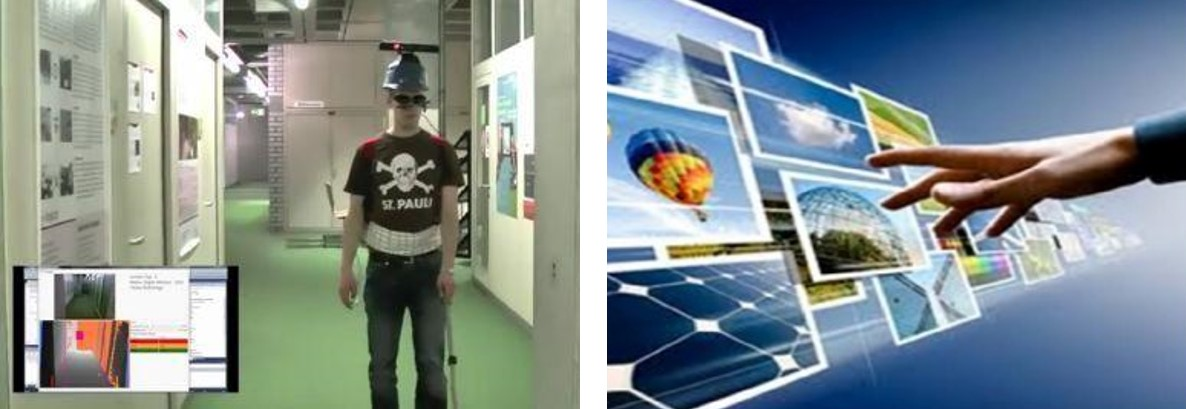
\includegraphics[width=\textwidth]{./figures/c1_apply_1.jpg}
    \begin{minipage}[t]{0.48\linewidth}
    \centerline{ \small (a) 盲人辅助设备}
    \end{minipage}
    \begin{minipage}[t]{0.48\linewidth}
    \centerline{ \small (b) 基于内容的海量图像检索}
    \end{minipage}
    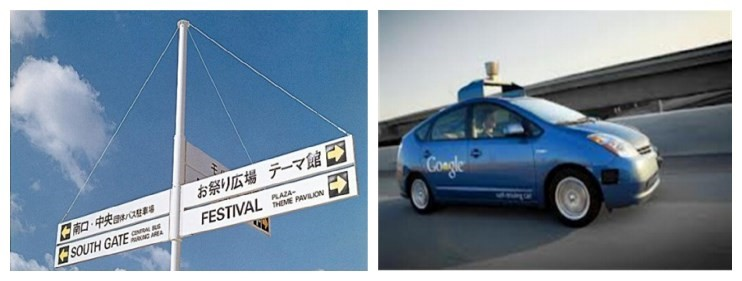
\includegraphics[width=\textwidth]{./figures/c1_apply_2.jpg}
    \begin{minipage}[t]{0.48\linewidth}
    \centerline{ \small (d) 国外旅游辅助}
    \end{minipage}
    \begin{minipage}[t]{0.48\linewidth}
    \centerline{ \small (e) 无人驾驶导航系统}
    \end{minipage}
    \caption{自然场景中文字检测与识别的应用}
    \label{fig.c1_apply}
    \end{figure*}

    在图像信息检索方面,通过计算机自动获取图像中可能存在的文字信息,可帮助计算机理解图像内容,实现对图像的自动标注,从而辅助图像搜索引擎,视频网站等工程场景的建设;在文档图像处理系统方面,可应用于淘宝、大众点评等门户网站,通过对顾客或商家上传的大量图像文件如发票、许可证书等进行文字检测和识别,可对图像进行自动判别和归类,以取代耗时耗力的人工审核;无人驾驶导航系统需要从无人驾驶汽车所处的道路环境中收集有效信息,并规划出从起点到终点的最优路径,而检测及提取出道路上标识牌中的文字信息,往往是无人驾驶导航系统能够安全、合法地行驶的必要条件;盲人辅助系统同样可通过文字检测获取标识牌及周围环境的文字信息,并通过文字识别将文字信息转换为语音或其它行驶的信息来辅助盲人获取环境信息。

    文字检测根据文字的存储媒介的不同又可分为不同类型如视频文字检测,自然场景图像文字检测等。其中,自然场景图像是指由人工拍摄而非计算机直接生成的图像。自然场景中拍摄的图像,其图像质量易受拍摄环境及拍摄条件的影响,背景较为复杂,图像中文字的字体、颜色及形态多变,这些因素都使得自然场景图像中的文字检测较为困难,呈现如图 \ref{fig.c1_problem} 所示的一些需要解决的难题:

    \begin{figure*}[!h]
    \centering
    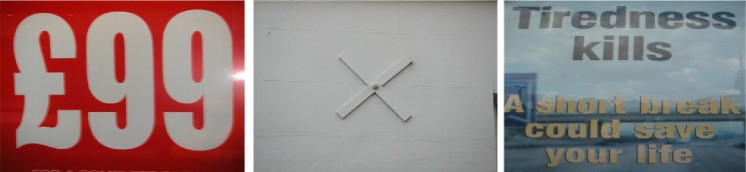
\includegraphics[width=\textwidth]{./figures/c1_problem_1.jpg}
    \begin{minipage}[t]{0.31\linewidth}
    \centerline{ \small (a) 多尺度}
    \end{minipage}
    \begin{minipage}[t]{0.31\linewidth}
    \centerline{ \small (b) 对比度低}
    \end{minipage}
    \begin{minipage}[t]{0.31\linewidth}
    \centerline{ \small (c) 不同颜色}
    \end{minipage}
    
\includegraphics[width=\textwidth]{./figures/c1_problem_2.jpg}
    \begin{minipage}[t]{0.31\linewidth}
    \centerline{ \small (d) 不均匀光照}
    \end{minipage}
    \begin{minipage}[t]{0.31\linewidth}
    \centerline{ \small (e) 排列方向多变}
    \end{minipage}
    \begin{minipage}[t]{0.31\linewidth}
    \centerline{ \small (f) 复杂背景}
    \end{minipage}
    \caption{自然场景文字领域的挑战}
    \label{fig.c1_problem}
    \end{figure*}

    这些挑战包括:复杂的自然场景:在自然环境中,有许多类似文字的人为目标,例如建筑、标志和绘画等。复杂的自然场景使得文字难以从背景中被区分开来;对比度过低:文字通常与背景有一定的对比度以便于人类识别。但是某些时候,文字可能与背景有非常相似的纹理和颜色,这时文字就难以被分辨出来;不均匀的光照:由于图像采集时的光照影响和图像采集设备的不均匀响应,会使图像中产生不均匀的光照,有时图像过暗,有时图像局部太亮。不均匀光照会引入颜色失真和恶化的视觉特征,从而导致错误的分割和检测结果;排列方向多变 自然场景图像中的文字不仅是水平或竖直排列,也会倾斜排列或者曲线排列。不同的排列方向使得文字检测需要考虑更多情况从而变得困难;多语种:世界上的语种数量较多,常见的有英文、中文、日文、阿拉伯文等。不同语种的文字有不同的特点,使得在进行文字检测识别时需要考虑很多不同情况。在自然场景中进行多语种文字检测识别是非常困难的;图像模糊和退化:由于图像采集时多变的工作条件和自动对焦的使用,散焦和模糊的自然图像时常会产生。图像压缩和解压也会影响图像的质量,特别是图像中的文字。图像散焦、模糊和退化会降低文字的锐度使得文字粘连在一起,使得文字分割检测变得更加困难;图像失真:当图像采集时图像采集设备如相机等的光轴不垂直于文字所在平面时会产生透视变形。文字包围盒不是矩形和字符扭曲,都会使失真的文字难以被检测出来。

    近年来在文字检测与识别领域,研究者们为解决上述难题做了大量的研究和探索,提出了大量的文字检测方法,检测结果也在逐年提高。但目前的方法在ICDAR 公开测试集上的测评结果表明,自然场景图像中的文字检测和识别效果仍有提升空间。

    \section{国内外研究现状}
    \esection{Related Work}

    自然场景图像中的文字检测和识别是计算机视觉领域的研究热点,国内外的很多学者在从事该方面的研究,他们也提出了很多的方法来解决这个问题,而Ye 等人\cite{Ye2015Text}对这些方法进行了调研和总结。 同时,在国际会议ICDAR 上举办了多次关于文字检测的比赛“Robust Reading”\cite{Karatzas2013ICDAR},自然场景中的文字检测及识别就是其中的一项比赛内容,不仅为从事文字检测方面研究的人提供了交流的机会,而且也反映了当时文字检测的最先进水平。

    自然场景图像中的文字检测方法按照其处理对象的不同,可分为基于纹理的方法和基于区域的方法:基于纹理的文字检测方法,把文字当作一种特殊纹理,通常通过局部颜色对比度、笔划滤波器、频域变换等方法来刻画文字的纹理特征。在确定纹理特征提取方式之后,往往会使用各种分类模型训练文字-背景分类器,以滑动窗的形式判断图像局部区域内是否包含文字,由此生成文字概率图。之后通过聚类或图像分割等方法取得候选文字行或文字区域,再经过后处理生成最终的检测结果。为检测不同尺寸的文字,基于纹理的方法往往需要在输入图像的不同尺度的图像上都进行同样的纹理特征提取和区域分类,或设计不同大小的纹理特征提取模板在同一个滑动窗内提取多次特征,并进行多尺度的结果融合。因此这类方法比较耗时;基于区域的文字检测方法,通常利用文字具有与背景差异明显且均一的颜色这一特征,从输入图像中提取出有限个数的候选文字区域,然后使用一些经验性的规则,或者提取区域的几何、纹理等特征,使用分类模型来滤除掉背景区域。基于区域的方法通常要比基于纹理的方法效率更高,因为基于区域的方法需要处理的区域数目有限。但这类方法的缺点在于,文字区域由于光照、遮挡、模糊等原因,内部颜色分布差异变大,或者边缘模糊,往往会在提取候选文字区域时被漏检,会直接影响最终检测结果。

    2010年,Epshtein\cite{Epshtein2010Detecting} 等人提出了笔画宽度变换(SWT)来计算图像中每个像素的笔画,基于像素笔画产生候选文字连通区域,去掉非文字连通区域就得到文字检测结果。笔画是组成文字的基本元素,通过计算笔画来检测文字是文字检测中非常有意义的研究进展;2011 年,Neumann 和Matas\cite{Neumann2011Text} 使用最稳定极值区域(MSER)作为候选文字区域,通过有效剪枝可以详尽搜索所有可能文字序列,并利用高阶文字属性(文字行)对候选区域进行区分从而确定文字区域;2012 年,Tu\cite{Tu2012Detecting} 等提出了一种检测自然图像中任意方向的文字的方法,他们使用SWT来获得候选文字连通区域,然后通过单个连通区域的分析和连通区域行的分析来去掉非文字部分,保留下来的连通区域就是文字检测的结果;2014 年,Yin\cite{Yin2013Robust}等设计了一个快速有效的剪枝算法来提取图像中的最稳定机制区域(MSER)作为候选文字连通区域,他们通过一个单链聚类算法将候选文字链接成候选文字行,这个聚类算法的距离权重和聚类阈值是通过一个自训练距离度量学习算法自动学习到的,通过贝叶斯模型利用字符分类器计算候选文字的后验概率,从而将文字检测出来;2015 年,Yu\cite{Yu2015Text} 等提出了一种基于边缘分析的文字检测方法,他们使用边缘重组来产生候选文字连通区域,然后通过单个连通区域分析、连通区域行分析对候选文字进行验证,得到最终的文字检测结果。

    近些年,随着深度学习\cite{Moral2010Foundations} 的兴起,它被广泛用于目标检测识别任务,例如手写字符识别、交通标志识别等,同时取得了非常好的结果,大大提升了目标检测识别的水平。鉴于深度学习的良好表现,许多人也将深度学习用于自然场景中的文字检测。2012 年,Wang\cite{Wang2012End}等提出基于深度学习的文字检测方法,他们利用一个包含2 个卷积层的卷积神经网络(CNN)对滑动窗进行分类,然后对重叠的窗口利用非极大抑制进行筛选就得到了文字检测结果;2014 年,Huang\cite{Huang2014Robust} 等使用MSER来产生候选文字连通区域,然后利用CNN计算每个候选文字连通区域属于文字的可能性,最后将属于文字的可能性比较高的连通区域串成文字行产生最终的检测结果;同时,他们提出来一种用于分开粘连文字的方法,基于CNN和滑动窗可以将一个连通区域中含有的多个粘连文字分开;2015年,Zhang\cite{Zhang2015Symmetry} 等利用滑动窗提取文字的对称性特征,从而计算每个像素属于文字行对称轴的概率,然后在此基础之上形成候选文字行,最后使用CNN将非文字部分去掉,剩下的就是文字区域;2016 年,Jaderburg\cite{Jaderberg2016Reading} 等首先利用一组互补的感兴趣区域(proposal)生成技术来确保检测阶段的高查全率,后续用高效的过滤阶段来提高查准率。最后用生成文本数据(synthetic text data)训练出的非常深的卷积神经网络来对检测阶段得到的包围框内的文字进行识别。

    ICDAR 2015 Competition on Robust Reading 是第五次关于自然场景中文字检测的国际比赛。该次比赛的获胜方法结果是R=0.80,P=0.90, 反映了目前自然场景中文字检测的最先进水平,这说明自然场景中的文字检测和识别目前还未达到可以商用的水平。近些年虽然获得了很多的关注和巨大的发展,但是自然场景图像中的文字检测和识别仍然是一个非常有挑战的问题。这是因为自然场景图像的背景一般比较复杂,其中各种语言、大小、字体、排列方向等的文字都可能会出现,由于光线条件影响,文字可能会过暗或过亮,还可能出现图像失真和退化,导致自然场景中的文字检测非常困难。

    \section{本文研究内容}
    \esection{Research Contents}

    本文针对自然场景图像中的文字检测方法展开研究,为解决文字边缘与背景边缘之间的粘连问题而提出一种基于边缘骨架切割的场景文字检测子。而为了改进文字定位包围盒重叠率不足的问题,又提出一种基于二叉树搜索的文字行定位优化框架。本文的主要研究内容如下:

    1)首先本文对现有的自然场景图像中的文字检测方法进行了充分的调研,对其中主流的基于区域和基于连通部件的这两类方法进行了分析和探讨,并举一些典型的方法来说明场景文字检测领域存在的难题。

    2)针对文字边缘与背景边缘之间的粘连问题,本文提出了一种基于边缘骨架切割的文字检测方法。首先对于输入的场景文字图片,利用结构化边缘检测方法得到边缘响应图,然后基于一系列像素强度值阈值,对边缘响应图进行分割,得到相应的二值化边缘图。接着在每个二值边缘图上,通过细化操作得到其边缘骨架图,并通过8 领域内像素点分析所找到的边缘骨架结点。而文字边缘与背景间的粘连点,就存在于这些边缘骨架结点中。因此断开粘连点得到候选的文字边缘骨架,然后经过形态学滤除来过滤掉大部分明显不是文字的边缘骨架,剩余的不易区分的非文字边缘骨架,可通过基于 CNN 的分类器来进一步滤除。最后基于非极大值抑制和文本行聚集操作,得到文本行定位结果。在公开数据集ICDAR以及MSRA上的实验结果证明了该方法在处理边缘粘连问题方面的有效性。

    3)针对文字定位包围盒与文字真实定位之间重叠率不足的问题,本章提出的是基于二叉树搜索的文本行定位矫正方法。首先对于输入的场景文字图片,利用边缘骨架切割检测子来提取粗略的候选文字包围盒定位结果。然而其定位结果存在重叠率不足的问题,为了进一步提高文字检测的精度,本文提出一种统计边缘响应算法,接着通过对统计边缘响应进行水平投影、求取梯度以及执行非极大值抑制等操作,以获得候选文本行。最后由生成的候选文本行中建立起二叉树型的搜索空间,并根据优化策略从搜索空间中找到最优的文本行定位结果。该结果即是经过优化后得到的文字细致定位结果,相比于边缘骨架切割检测子所得到的粗略定位结果而言,其文字检测的精度得到了大幅提升。在ICDAR系列测试集以及谷歌街景数据集SVT 上,我们将本章提出的方法与其它先进方法以及边缘骨架切割检测子都做了对比实验。实验结果验证了该方法的确优化了文字包围盒的定位效果。

    \section{论文的组织结构}
    \esection{Thesis Structure}

    本论文是根据提出、分析然后解决问题的思路来组织内容的,后续的章节安排如下所示:

    第一章的内容是绪论部分。本章首先对自然场景图像中的文字检测这个研究方向的背景与意义进行介绍,然后对这个领域内的研究现状及其问题进行了调研和分析,接着概述了本论文的研究内容以及组织结构。

    第二章是论文的相关理论与技术。主要介绍了自然场景图像中的文字检测方法的两大类主流方法:基于区域的方法和基于连通部件的方法。然后各举一些经典方法以分析每类方法的优缺点,从而奠定本文研究工作的理论基础。

    第三章是基于边缘骨架切割的文字检测方法。本章首先引出边缘粘连问题这个文字检测领域中的难题,然后开始介绍针对该难题所提出的边缘骨架切割文字检测子的具体实现:包含该方法的原理、步骤以及详述。最后通过在公开数据集上将该方法与其它先进方法进行对比试验来验证方法的精度和时间性能。

    第四章是基于二叉树搜索的文字行定位优化方法。本章首先指出第三章提出方法可能存在的不足:即文字包围盒的定位重叠率达不到要求,然后详述基于二叉树搜索的文字行定位矫正算法来作改进。最后利用在多个数据集上的实验方法来验证了本章提出方法在文字包围盒定位精度上的提升。

    第五章是结论和展望:主要是总结全文,并展望了接下来的研究工作。


